\section{Background}
We will start with formal definitions of auto-tuning and stencil computation, followed by a brief introduction to GPU architecture and its programming model. Then we end the section with details on selected algorithms.

\subsection{Auto-tuning}
Given a program with n tunable parameters, we call a tuple of values $(x_1, ..., x_n)$ corresponding to each parameter a \emph{configuration}. The set of all possible configurations is called a \emph{parameter space} or \emph{search space}. Auto-tuning  is the problem of finding the configuration that gives the best performance. Although the performance metric can be any values of interest, the most common metric is the running time (lowest is best), and so do this project.

There are various approaches to auto-tuning, which could be classified into 3 broad categories \cite{inpar2012}:
\begin{description}
	\item[Model-based optimization] involves analytically constructing a performance model specific to the underlying hardware and does code transformation accordingly. However, such models are generally difficult to build.
	\item[Empirical optimization] searches for the best configuration by measuring the actual running time of a subset of all configurations. Usually, the subset is determined on-the-fly with a search method. If the subset is the whole search space itself, then this equals to exhaustive search. This approach takes considerably more time than the model-based approach, and there is a tradeoff between faster running time and better results.
	\item[Predictive optimization] combines the first two approaches, enhancing the empirical optimization by modeling/predicting the running time instead of benchmarking on real hardware. In this project we will use this approach and use machine learning algorithms for the prediction part.
\end{description}

\subsection{Stencil Computation}
Stencil computation is used in wide range applications from solving system of Partial Differential Equations (PDEs) to filtering in image processing. It iterates over timesteps and performs stencil operations on all points in a grid in each iteration. Stencil operation on a point updates its value to a linear combination\footnote{In other words, weighted sum} of its nearest neighbors, within a fixed distance, and sometimes itself. An example 3D 25-point stencil is shown in Figure~\ref{fig:25-point_stencil}. We will use this stencil in our benchmark application.

%\begin{figure}[!th]
%\centering
%\begin{minipage}{.5\textwidth}
%\centering
%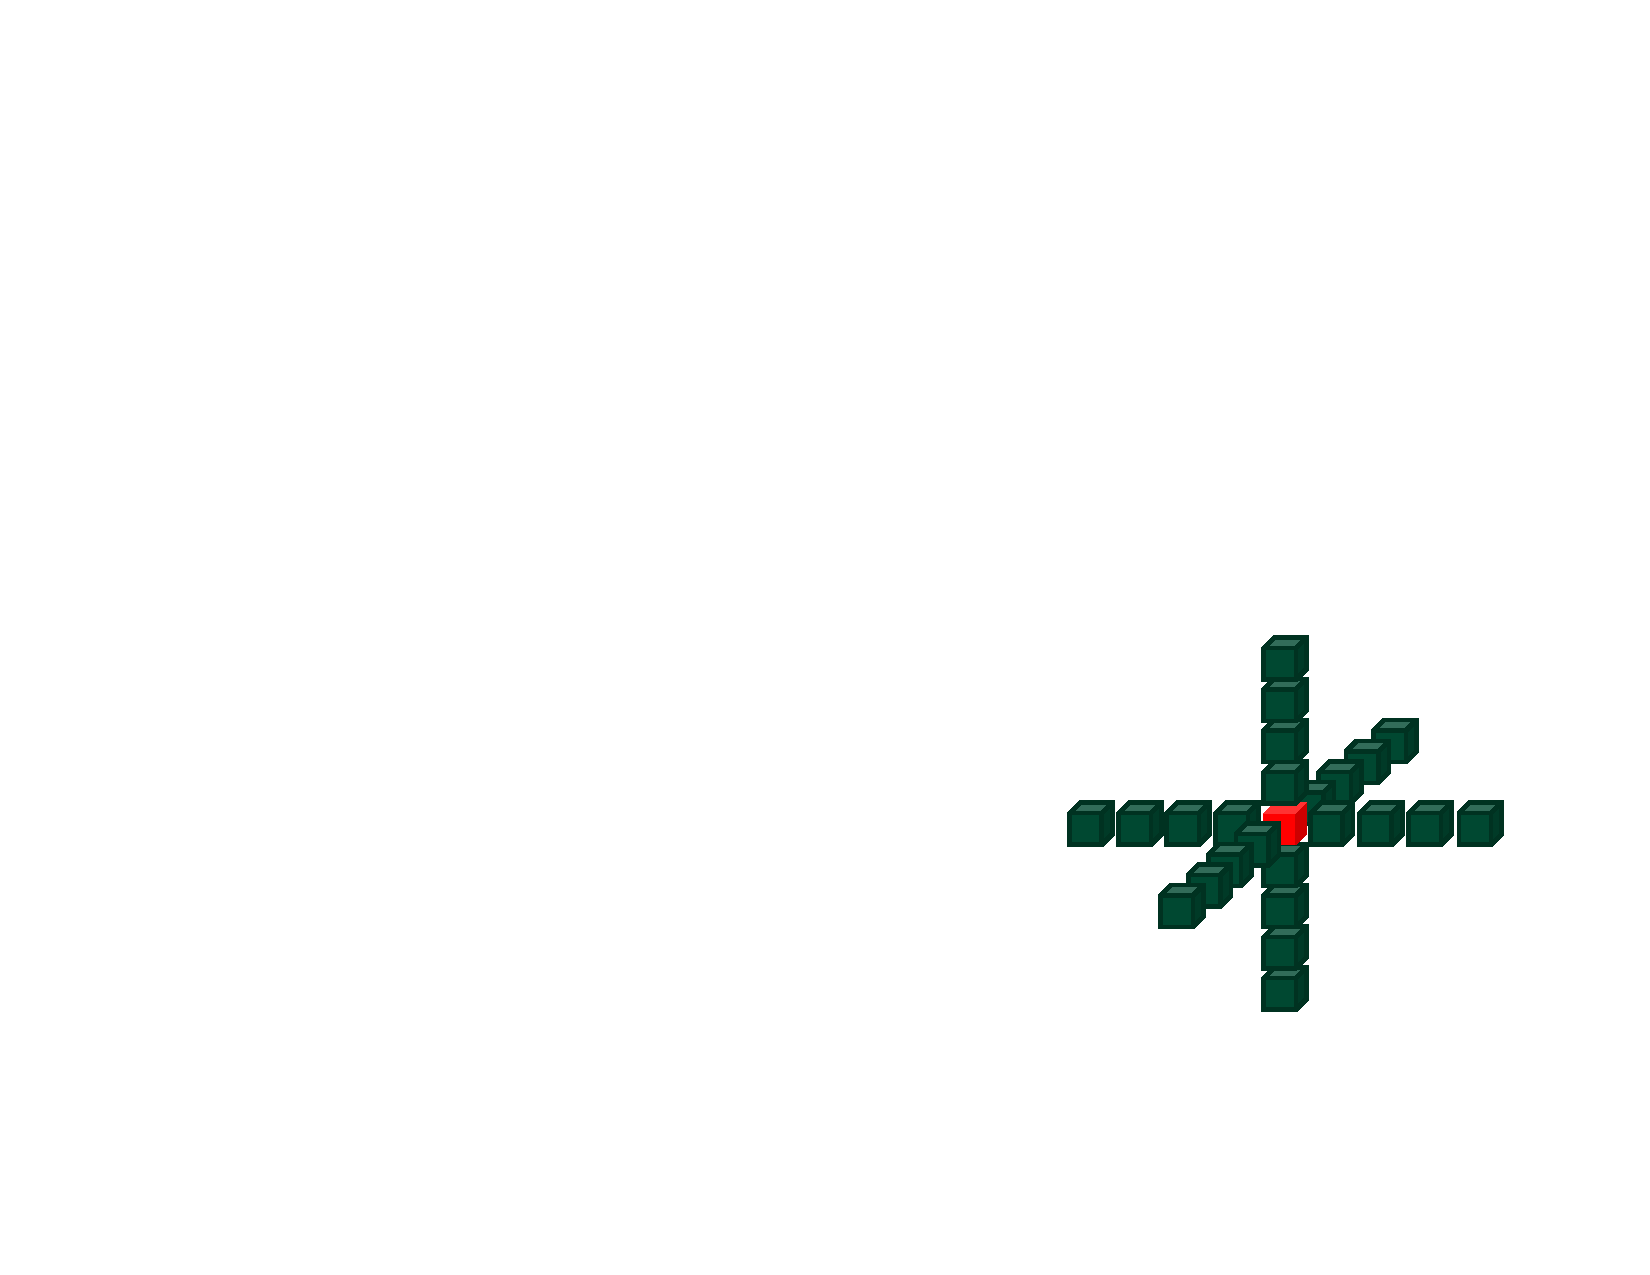
\includegraphics[width=0.25\textwidth]{./images/25-point-stencil.pdf}
%\caption{Illustration of a 3D 25-point stencil (4 neighbors in each direction). (Courtesy of NVIDIA)}
%\label{fig:25-point_stencil}
%\end{minipage}
%\begin{minipage}
%\centering
%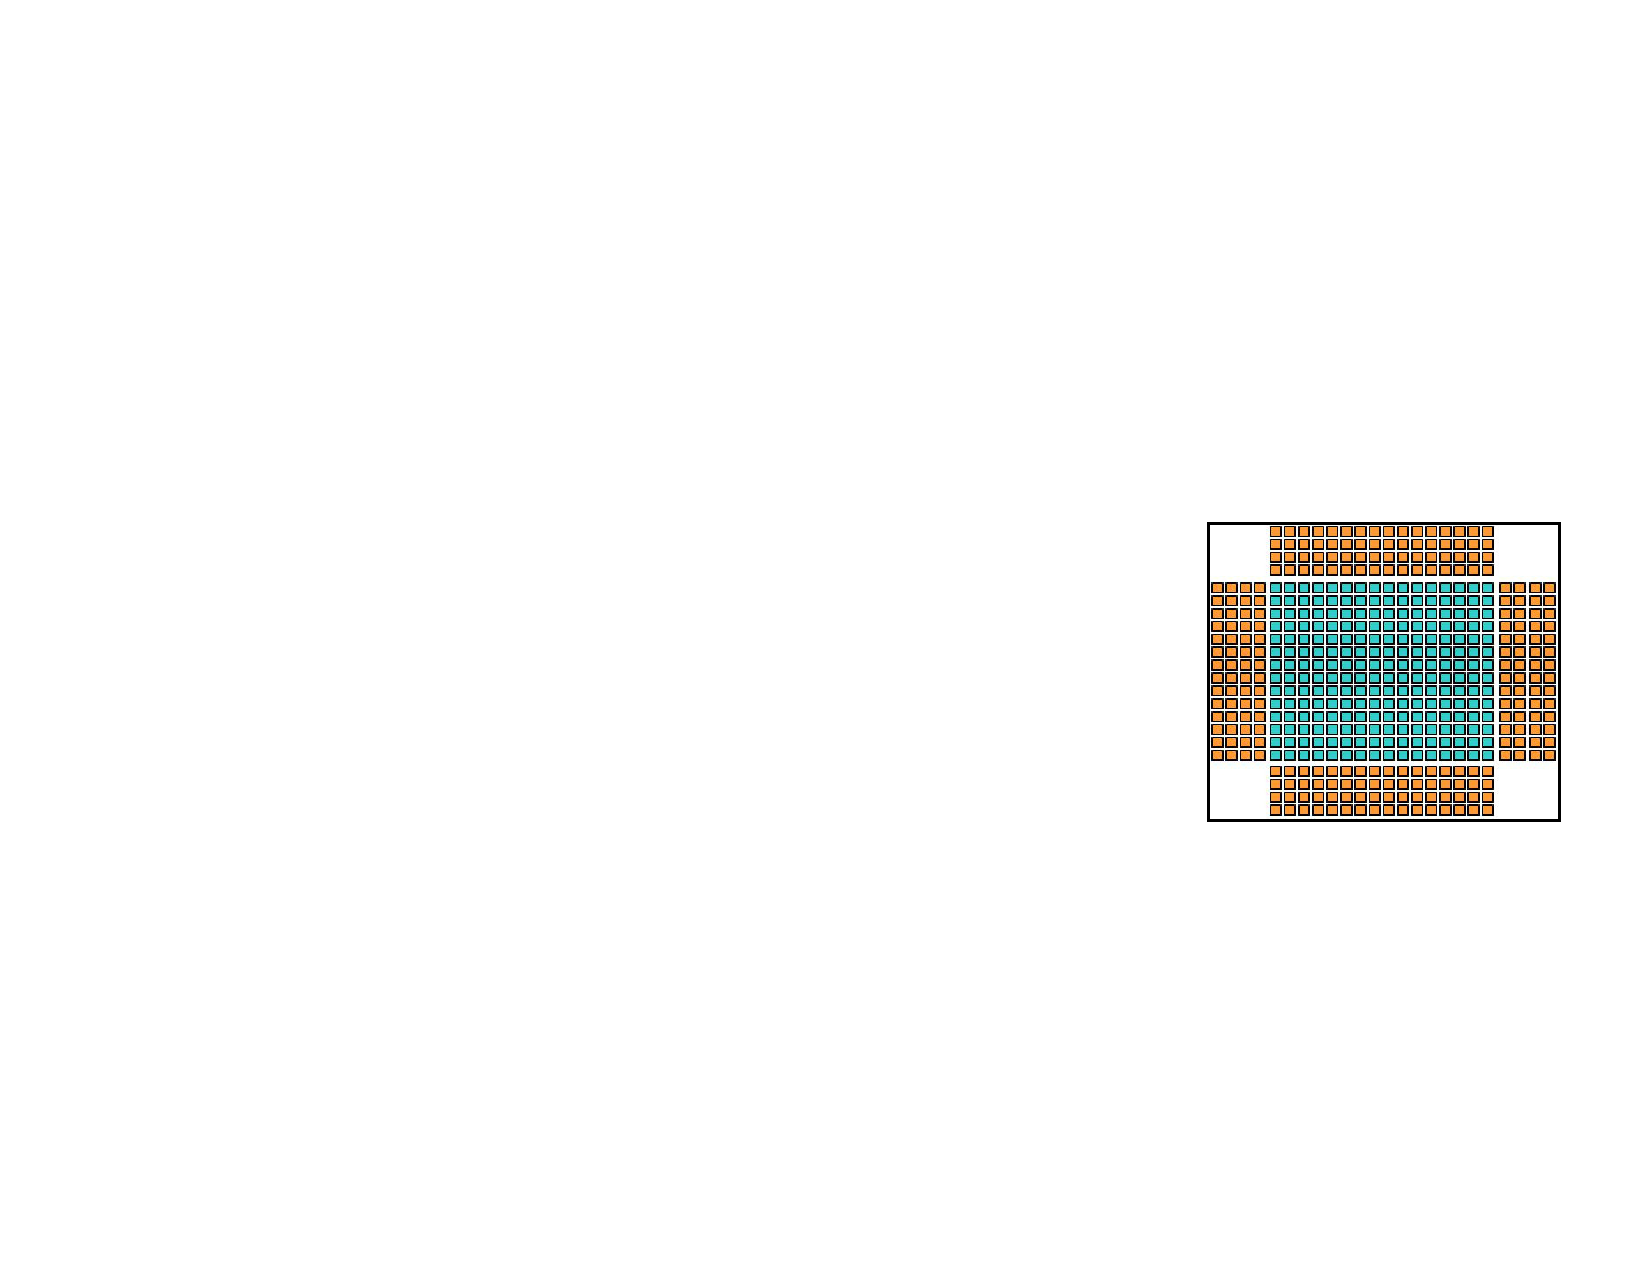
\includegraphics[width=0.25\textwidth]{./images/gpu-architecture.pdf}
%\caption{NVIDIA GPU architecture (Courtesy of NVIDIA)}
%\label{fig:gpu-arch}
%\end{minipage}
%\end{figure}

\begin{figure*}[!t]
\centering
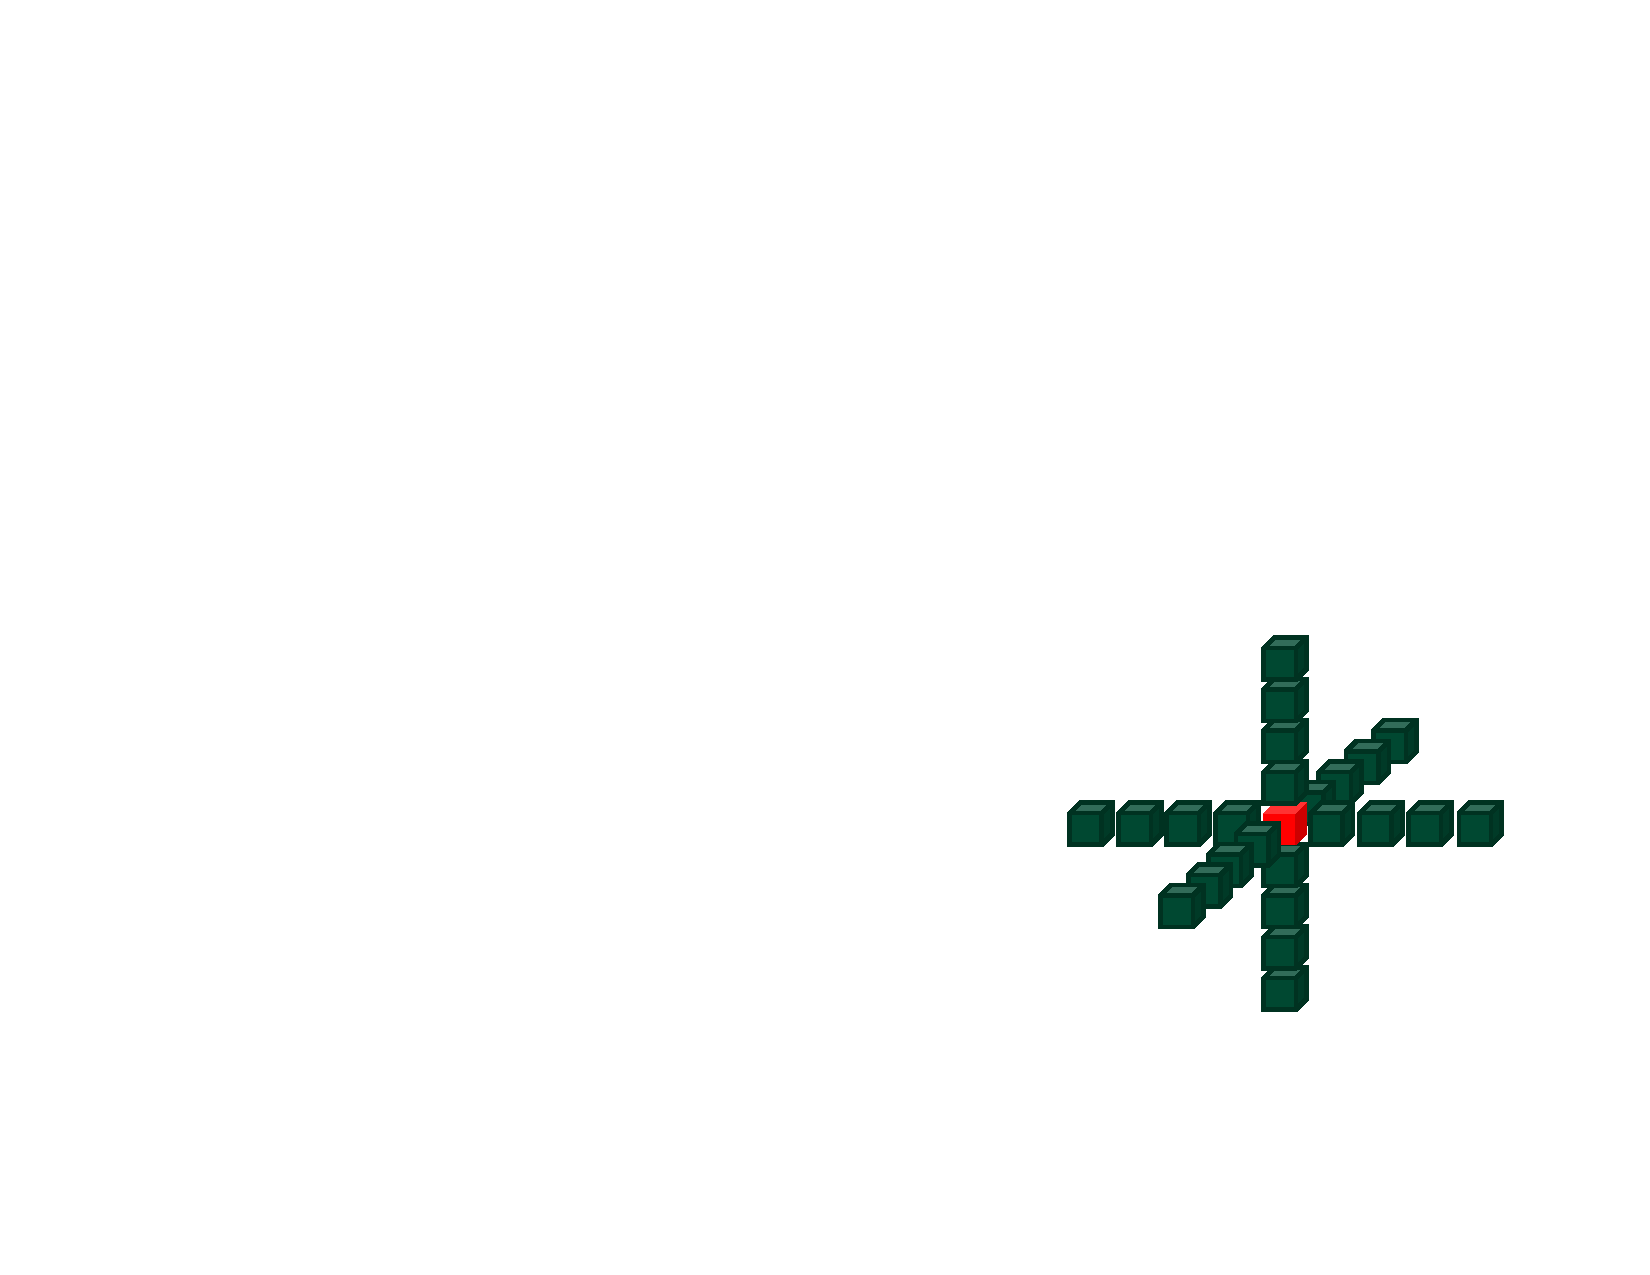
\includegraphics[width=0.25\textwidth]{./images/25-point-stencil.pdf}
\caption{Illustration of a 3D 25-point stencil (4 neighbors in each direction). (Courtesy of NVIDIA)}
\label{fig:25-point_stencil}
\end{figure*}

Stencil computation is mostly bandwidth-bound, since they rely on many points around while the computation is trivial.

\subsection{NVIDIA GPU and CUDA Programming Model}
GPU (Graphical Processing Unit) is a massively parallel processor that was originally designed for just display purpose. With the introduction of programming frameworks that allows programmers to program general-purpose application on GPUs more conveniently, graphic cards quickly became one of the most popular hardware accelerators nowadays. Among all vendors, NVIDIA GPUs are the most popular and widely available.

Figure \ref{fig:gpu-arch} shows the architecture of an NVIDIA GPU. An NVIDIA GPU consists of many SIMD (Single Instruction Multiple Data) cores, dubbed Streaming Multiprocessors, and its own high-bandwidth DRAM memory. Each core has a large register file and a user-managed cache called \textbf{shared memory}. There are three types of out-of-core memory: global memory, constant memory, and texture memory. Global memory is the largest one and is used in general purpose. The latter two are read-only.

\begin{figure*}[!t]
\centering
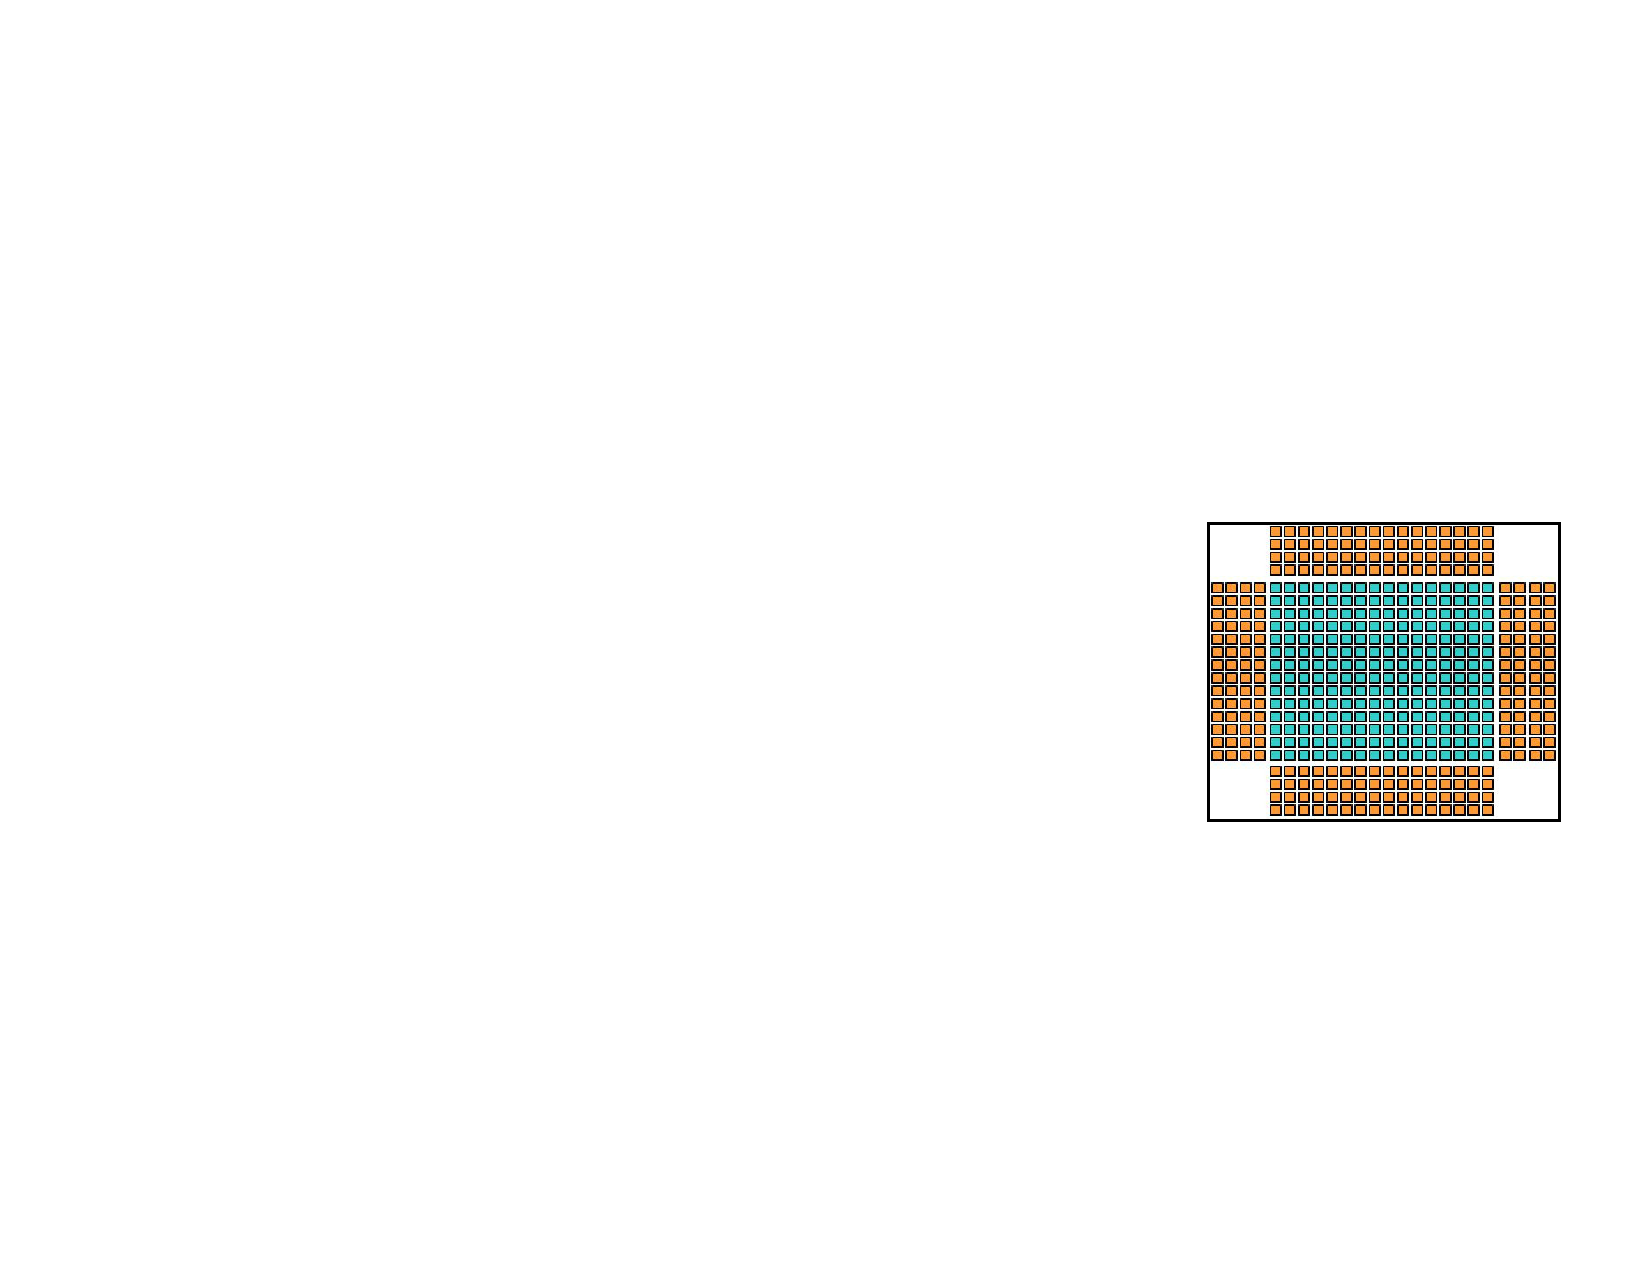
\includegraphics[width=0.25\textwidth]{./images/gpu-architecture.pdf}
\caption{NVIDIA GPU architecture (Courtesy of NVIDIA)}
\label{fig:gpu-arch}
\end{figure*}

The programming model for NVIDIA GPUs is called CUDA (Compute Unified Device Architecture). To program on a GPU, one needs to write a normal CPU \emph{`host'} code that calls a separate CUDA \emph{`kernel'}\footnote{Not to be confused with kernels in Statistics} code, which is simply a function to be executed simultaneously on GPU cores.

A set of all threads that is used to execute a kernel is referred to as a ``grid" in CUDA context. For each grid, the threads are divided into groups called thread blocks (for scalability reasons ..cite CUDA Programmming Handbook). Threads in the same block will be executed on the same GPU core, and will be able to share resources and synchronize. The block size affects the resources usage on a core and determines how many threads will be able to execute on the whole GPU device in total, and thus it is one of the most important tuning parameters of a GPU program.

Given that a stencil computation is bandwidth bound, the keys to optimize its applications are simply:
\begin{enumerate}
	\item Optimizing for highest memory bandwidth by
		\begin{enumerate}
			\item Coalescing memory reads from global memory.
			\item Design load and store pattern to minimize extra reads from global memory. For example, use shared memory to share data among threads in the same block, and order the usage pattern so that we don't need to load the same data again later in the computation.
		\end{enumerate}
	\item Utilizing as many computing resources as possible
\end{enumerate}

\subsection{Machine Learning in Auto-tuning Stencil Computation}
There are several auto-tuning researches on stencil computation on GPUs, but they don't utilize Machine Learning. Datta et al.\ and Kamil et al.\ explained a thorough framework to auto-tune stencil computation on various multicore architectures including NVIDIA GPUs. They used empirical optimization with iterative greedy search algorithm with heuristics. \cite{datta08, datta09, shoaib10} Zhang and Mueller recently explored auto-tuning of 3D stencil computatoin exclusively on GPUs, including GPU clusters. They exhaustively tested all configurations. \cite{zhang12}

In fact, there are few auto-tuning project on GPU that even uses machine learning. To be appear in the inaugural Innovative Parallel Computing (InPar) 2012 is a work on predictive auto-tuning on GPU by Bergstra et al.\ \cite{inpar2012} They used Boosted Regression Tree (BST) to predict program's performance and used hill-climbing (HC) search algorithm to find the best configuration. Their benchmark application was a simple spatial image filter called Filterbank correlation. They found that the predicted running times correlate very well with the results from their actual runs across 5 models of NVIDIA GPUs. They also asserted that the auto-tuning should be input-dependent, that is choosing kernels according to each input configuration.

Ganapathi et al.\ took an interesting approach in tuning stencil computation on multicore architectures, although GPU was not included. \cite{KCCA} Having set the desired performance metrics to be both energy and speed, she opted for a rather compute-intensive machine learning algorithm called Kernel Canonical Correlation Analysis (KCCA). The key idea is to project the set of configurations and the set of measured corresponding metrics onto a space that they correlate the most, and then project the best configuration of the test set onto that space, find nearest neighbors in the projected space, and then generate new (much smaller) set of configuration to be searched empirically for the best parameter. The performance the auto-tuning was able to achieve is within 1\% of and up to 18\% better than a human expert.

Observing that the BRT and KCCA algorithms perform well, I chose to study 2 regression tree algorithms and 2 kernel algorithms: (Gradient) Boosted Regression Tree, Random Forest, Kernel Ridge Regression, and Kernel Canonical Correlation Analysis.
\begin{description}
\item[Regression Trees] Regression Trees predict by recursively dividing input space to constant region. They are interesting to auto-tuning because they are non-parametric. That is, they don't need to know the probability distribution of the latent variable. Apart from quick decision time, the splitting condition can help in learning what parameters is crucial in tuning, which is always good to know regardless of how obvious they are. However, they do have drawbacks. Regression trees have high variance since each different decision at the splitting node can lead to totally different conditions later on down the tree. However, this can be avoided by additive algorithms. \textbf{\emph{Boosted Regression Tree}} is a committee-based algorithm that tries to create a strong learner from multiple weak learners. It iteratively combines regression trees from learning samples that are weighted so that the ones that were previously classified wrong has more weight (Learning from mistakes). \textbf{\emph{Random Forest}} is another way by combining random trees together.
\item[Kernel Canonical Correlation Analysis] is a kernelized version of Canonical Correlation Analysis.\cite{KICA} It is similar to PCA in essence. The algorithm is previously mentioned in last paragraph. The projection can be viewed as discovering the generating factors that lies behind two sets of data. For example, in auto-tuning configurations and observed running times are the two sets of data and the maximal correlation projection can be considered the projection of all deciding hardware and application constraints summarized in just one dimension. I'm very interested and intrigued by this. Thus, I include it here even though it seems to be an overkill for this problem. (Solving KCCA equals to solving generalized eigenvector problem, thus it has $O(n^3)$ complexity.)
\item[Kernel Ridge Regression] I add this
\end{description}



% Add KCCA if I can use it..
% Add amik paper if end up using analytic model
